%\section{Dealing with silent data corruption}
Different from crash failures, which crashes a process, silent data corruption allows a faulty process to continue to completion but generate incorrect results. To deal with $f$ failures of this type, $(2f+1)$ replicas are needed, and voting is involved at the end to identify the correct results. For example, when at most 1 silent data corruption could occur, 3 replicas are necessary and sufficient to tolerate the failure. In the following, we will focus on tolerating one silent data corruption per data split. 

Soft Replication can deal with silent data corruption with potentially higher efficiency and less resource requirement compared to traditional replication techniques. For each split, Soft Replication associates 2 fast replicas with 1 slow replica. To save energy, the slow replica executes at a potentially lower rate than the 2 fast replicas, and dynamically speeds up if a fast replica fails. 

\subsection{Notations}
Let $W$ denote the required workload to process one data split, which is often the unit of transfer from disk to main memory. Let $\sigma_{max}$ denote the maximal execution rate, then $R_{min}=\frac{W}{\sigma_{max}}$ is the minimal response time. Let $\overline{R}=(1+\alpha)R_{min}$ $(0\leq \alpha \leq 1)$ denote the fault-tolerant response time. Let $\lambda$ denote the failure rate, and $f(t)$ denote the failure density function. Let $E(\sigma, [t_1, t_2])$ denote the energy consumption of a process when executing at rate $\sigma$ for an interval from $t_1$ to $t_2$.

To deal with silent data corruption, the Soft Replication model entails three execution rates:
\begin{itemize}
	\item $\sigma_{m}$, the execution rate of the fast replicas 
    \item $\sigma_{b}$, the execution rate of the slow replica before a fast replica fails
    \item $\sigma_{a}$, the execution rate of the slow replica after a fast replica fails
\end{itemize}

\subsection{Response time}
Assuming there is at most one silent data corruption, three scenarios need to be considered, i.e., no failure, one fast replica fails, or the slow replica  fails.

In the first scenario, where no failure occurs, the response time is determined by the fast replicas, as $t_r^m=\frac{W}{\sigma_m}$.

In the second scenario, 
where the slow replica fails, the fast replicas are not impacted, and thus the response time is also determined by the fast replicas, as in the first scenario. Therefore, $t_r^m=\frac{W}{\sigma_m}$.


In the last scenario, where one fast replica fails, the response time is determined by the slow replica. The work completed by the slow replica before the fast replicas complete is $w_b = \sigma_b \times t_r^m$. Then the remaining work for the slow replica to complete is $w_a = W - w_b$. As a result, the total response time by the slow replica is $t_r^s = t_r^m + \frac{w_a}{\sigma_a} = \frac{W(\sigma_m + \sigma_a - \sigma_b)}{\sigma_m \sigma_a}$.



\subsection{Energy consumption}
To calculate energy consumption, we also use the power model described in Section~\ref{sec:power_model}.
Corresponding to the three scenarios in the above response time analysis, the energy consumption also falls into three cases. 

If no failure occurs, the energy consumption of the three replicas weighted by its probability is
\begin{equation}
\begin{split}
E_1 = & (1 - \int_{0}^{t_r^m} f_m(t)dt)^2 \times (1 - \int_{0}^{t_r^m} f_s(t)dt) \times \\
      & \{2E(\sigma_m, [0, t_r^m])+E(\sigma_b, [0, t_r^m])\}
\end{split}
\end{equation}

If one fast replica fails, the energy consumption weighted by its probability is 
\begin{equation}
\begin{split}
E_2 = & 2(1 - \int_{0}^{t_r^m} f_m(t)dt) \times 
(1 - \int_{0}^{t_r^m} f_s(t)dt) \times \int_{0}^{t_r^m} f_m(t)dt \times \\       & \{2E(\sigma_m, [0, t_r^m]) + E(\sigma_b, [0, t_r^m]) + E(\sigma_a, [t_r^m, t_r^s])  \}
\end{split}
\end{equation}

If the slow replica fails, the energy consumption weighted by its probability is 
\begin{equation}
\begin{split}
E_3 = & (1 - \int_{0}^{t_r^m} f_m(t)dt)^2 \times \int_{0}^{t_r^m} f_s(t)dt \times \\  & \{2E(\sigma_m, [0, t_r^m])+E(\sigma_b, [0, t_r^m])\}
\end{split}
\end{equation}

All in all, the total energy consumption is the sum of the above three, i.e., $E_{total}=E_1 + E_2 + E_3$. 

\subsection{Optimization}
Similar to dealing with crash failures, an optimization problem can be formulated for dealing with silent data corruption to derive the optimal values for the three execution rates, in order to minimize the total energy consumption while meeting response time constraint. 

\begin{equation}
\begin{alignedat}{2}
\min_{\sigma_m,\sigma_b,\sigma_a} \qquad  & E_{total} \\
s.t.  \qquad          & 0 \leq \sigma_m \leq \sigma_{max} \\
                      & 0 \leq \sigma_b \leq \sigma_m \\
                      & \sigma_b \leq \sigma_a \leq \sigma_{max} \\
                      & max(t_r^m, t_r^s) \leq \overline{R}
\end{alignedat}
\end{equation}

The first constraint says the execution rate of the fast replicas should observe the physical processor limit. The second constraint indicates that the slow replica should not exceed the execution rate of the fast replicas. The third constraint ensures that the slow replica could speed up after detecting a failure. The last constraint guarantees that the deadline is met even in the case of failure.



\subsection{Performance evaluation}

\begin{figure*}[!t]
	\begin{center}
		\subfigure[Sensitivity to failure rate. $W=100$ hours, $\alpha=0.25$, $\rho=0.5$.]
		{
			\label{fig:silent_lambda}
			\includegraphics[width=0.45\textwidth]{figures/silent_lambda}
		}
		\subfigure[Sensitivity to static power ratio. $W=100$ hours, $\alpha=0.25$, $MTBF=5$ years.]
		{
			\label{fig:silent_power}
			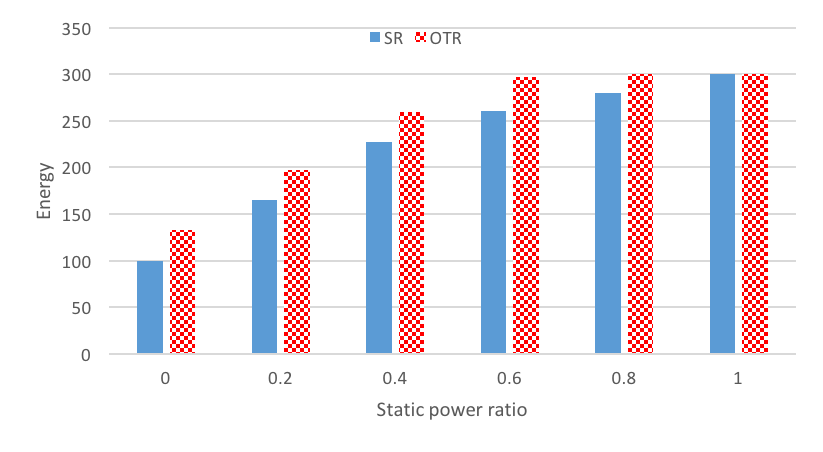
\includegraphics[width=0.45\textwidth]{figures/silent_power}
		}
		\subfigure[Sensitivity to laxity. $W=100$ hours, $\rho=0.3$, $MTBF=5$ years.]
		{
			\label{fig:silent_time}
			\includegraphics[width=0.45\textwidth]{figures/silent_time}
		}
        \subfigure[Sensitivity to workload. $\alpha=0.25$, $\rho=0.5$, $MTBF=5$ years.]
		{
			\label{fig:silent_w}
			\includegraphics[width=0.45\textwidth]{figures/silent_w}
		}
	\end{center}
	\caption{Comparison between Soft Replication and Traditional Process Replication for energy consumption under a single silent failure.}
	\label{fig:silent_eval}
\end{figure*}




